\documentclass{article}
\usepackage[utf8]{inputenc}
\usepackage[spanish]{babel}
\usepackage[hidelinks]{hyperref}
\usepackage{setspace}
\usepackage{graphicx}
\usepackage{float}
\usepackage[hidelinks]{hyperref}

\usepackage[compact]{titlesec}
\usepackage{geometry}
\geometry{
    a4paper,
    total={170mm,257mm},
    left=30mm, % entre 25-35
    right=30mm, % entre 25-35
    top=30mm, % no más de 30
    bottom=30mm, % no más de 30
}

\usepackage{fancyhdr}
\pagestyle{fancy}
\fancyhf{}
\lhead{}
\rhead{Bárbaros Software S.A.}
\rfoot{\thepage}
\lfoot{Plan de gestión, análisis, diseño y memorial del proyecto KeyPaX}
\renewcommand{\footrulewidth}{0.4pt}

\setlength{\parindent}{2em}
\setlength{\parskip}{1em}

\begin{document}

\begin{titlepage}
    \centering
    \vspace*{\fill}

    \vspace*{0.5cm}

    \Huge
    \textbf{Plan de gestión, análisis, diseño y memorial del proyecto KeyPaX}

    \vspace*{0.5cm}

    \huge
    Bárbaros Software S.A. (Grupo 3)

    
\includegraphics[height=5cm]{../images/logo.jpg}

    \begin{Large}
        Carlos Bellvis, 755452\\
        Jorge Bernal, 775695\\
        Jorge Borque, 777959\\
        Arturo Calvera, 776303\\
        Andoni Salcedo, 785649\\
        Javier Vela, 775593\\
    \end{Large}

    \vspace*{1cm}

    \large
    \href{https://github.com/UNIZAR-30226-2021-03}{Organización GitHub: https://github.com/UNIZAR-30226-2021-03}

    \vspace*{\fill}

\end{titlepage}

\pagebreak

\tableofcontents

\pagebreak

\section{Introducción}

\section{Organización del proyecto}

El equipo del proyecto está formado por los 6 integrantes del grupo. 
Para dividir el trabajo y las responsabilidades se han formado 2 grupos iniciales, 
de acuerdo con las capacidades y conocimientos individuales. 
Además, se ha designado como \textbf{director del proyecto} a \textbf{Arturo Calvera}, 
sobre el cual recae la gestión de los equipos de trabajo y las responsabilidades de los mismos.

\begin{itemize}
    \item \textbf{Equipo \textit{Backend}}:
    \begin{itemize}
        \item Responsable: Arturo Calvera.
        \item Función: Desarrollo del \textit{backend} del sistema.
        \item Integrantes: Arturo Calvera, Andoni Salcedo.
    \end{itemize}
    \item \textbf{Equipo \textit{Frontend}}:
    \begin{itemize}
        \item Responsable: Javier Vela.
        \item Sub-equipos: El equipo dedicado a la vista del sistema se divide para el desarrollo de las dos interfaces.
        \begin{itemize}
            \item \textbf{Equipo Web}:
            \begin{itemize}
                \item Función: Desarrollo del \textit{frontend} web del sistema.
                \item Integrantes: Jorge Bernal, Javier Vela.
            \end{itemize}
        \item \textbf{Equipo Android}:
            \begin{itemize}
                \item Función: Desarrollo de la aplicación cliente del sistema para dispositivos Android.
                \item Integrantes: Carlos Bellvis, Jorge Borque.
            \end{itemize}
        \end{itemize}
    \end{itemize}
    \item Se contempla la posibilidad de modificar dicha división en equipos para adaptarse a las necesidades que surjan durante el desarrollo del proyecto.
\end{itemize}

\section{Plan de gestión del proyecto}

\subsection{Procesos}

\subsubsection{Procesos de inicio}

Para la identificación y asignación de recursos a utilizar, se han puesto en común los conocimientos
tecnológicos de cada integrante del grupo realizando así un sondeo de las opciones disponibles, el 
grado de familiarización con las tecnologías y las preferencias individuales de los desarrolladores. 

Respecto a los servidores en \textit{cloud} a utilizar para el despliegue del sistema, se barajaron
los servicios de \textit{cloud} \textit{Amazon Web Services y MIcrosoft Azure}.
El criterio de elección se ha basado en el estudio del impacto a nivel global de la empresa, es decir,
grado de utilización en el mundo empresarial y la cantidad de servicios ofrecidos gratuitamente por.
Finalmente, teniendo en cuenta los criterios anteriores, se decide crear una cuenta en \textit{AWS} 
siendo así \textit{Amazon} el proveedor de cloud para el proyecto.

\pagebreak
En relación a la base de datos, se ha decidido usar una base no relacional debido al grado de flexibilidad
de modelo de datos que ofrece frente al modelo típico relacional. Como SGBD se ha escogido \textit{MongoDB}.
Se ha creado una cuenta en \textit{MongoDB Atlas} el cual permite crear una base de datos remota accesible
por el sistema.

En cuanto a la formación inicial de los integrantes, se han tenido en cuenta en el reparto de responsabilidades 
los conocimientos de los desarrolladores, sin embargo, todos los desarrolladores dedicarán tiempo de manera individual 
en autoformación con tutoriales y documentación sobre las tecnologías a usar en el desarrollo del sistema.
Además, todos los integrantes del grupo se han comprometido a formar a sus compañeros en las areas que conozcan
a medida que surgan dudas durante el desarrollo del sistema.


\subsubsection{Procesos de ejecución y control}

Las comunicaciones entre los miembros del grupo de trabajo se realizarán principalmente a través de la herramienta 
de comunicación \textit{WhatsApp}, mediante la cual se concretan los horarios de trabajo 
y se informa acerca de actualizaciones puntuales en las tareas asignadas a cada miembro para que todo el equipo quede 
informado de cómo avanzan los distintos componentes del trabajo. 
Además, las reuniones semanales de puesta en común del trabajo se realizarán utilizando la herramienta de videoconferencia 
\textit{Google meet}. Esta última será el principal medio de comunicación del grupo. 
Destacar que pese a la división de trabajo previa, se intenta trabajar de manera conjunta por videoconferencia, 
de manera que se puedan poner en común y resolver problemas en la medida en que surjan.

En cuanto al registro de las decisiones tomadas en las reuniones, se plasmarán en actas gestionadas 
por Javier Vela. Respecto al almacenamiento de estas actas se realizará en un directorio remoto en \textit{GitHub}

Partiendo de la división inicial del grupo en equipos de trabajo detallada en el punto 2, los responsables
de cada equipo de trabajo se encargarán de monitorizar el avance de sus respectivos módulos, determinar 
las tareas a realizar, asignar dichas tareas a los desarrolladores y marcar límites temporales y prioridades para cada tarea.
En cuanto al trabajo de documentación del los avances sobre el código, todos los desarrolladores serán responsables 
de registrar los mismos en las \textit{Wikis de GitHub} habilitadas para ello en cada repositorio de código.
Así mismo, los desarrolladores tendrán que rellenar una tabla de control de esfuerzos para registrar su trabajo y 
cumplir con el resto de planes especificados más adelante.

De la resolución de disputas se encargará el miembro Jorge Bernal, quien actuará como mediador cuando surgan conflictos en cualquier
ámbito del desarrollo del proyecto, pudiendo acudir a este en cualquier momento si se necesitase de su ayuda.
%% IGUAL SOBRA ?? relativas a la implementación de las diferentes partes del trabajo, ya bien sean de código o completar documentación. Resaltar que puesto que somos un grupo muy compenetrado, la labor de gestionar el equipo no es realmente complicada. El éxito de nuestro proyecto se basa en la paciencia, el respeto por los compañeros de equipo y la alta implicación por querer aprender acerca de aspectos que no dominamos.

Respecto a la monitorización y control del progreso del proyecto, todas las semanas se realizará una reunión conjunta
de control en una hora y día fijadas a la cual asistirán todos los mismbros del grupo para exponer los avances realizados
durante la semana y poder determinarse el estado del proyecto y las siguientes tareas a desarrollar. Así mismo, tal y como
se detalla en el punto 3.2.3 existen mecanismos para asegurar la calidad del producto y detectar posibles de rendimiento en 
el completado de las tareas.

%%Centrándonos más en la parte de monitorización y estado del proyecto, la gestión de estos aspectos se podría decir que es semanal, puesto que va sincronizada con las reuniones semanales que, decidiendo por mayoría, quedamos en que tuviesen lugar todos los martes de 12:00 a 14:00. De este modo, estas dos horas nos sirven para poner encima de la mesa todo el trabajo realizado durante la semana, de tal manera que todos los miembros del grupo nos enteramos de como van avanzando las diferentes partes del proyecto y, en función del plan de trabajo a completar establecido la semana anterior, se toman decisiones del tiempo a invertir para terminar el trabajo atrasado. Por otra parte, fijándonos en la carga de trabajo propuesta para la semana anterior y el porcentaje del mismo que hemos completado, proponemos un plan de trabajo a completar para el martes de la semana siguiente. Estimamos el poder completar cada semana un 10\% del trabajo total.

La entrega de resultados se hará de manera continua de tal forma que el cliente pueda ir viendo el progreso del proyecto. 
El equipo se compromete a entregar los resultados del mismo en los plazos preestablecidos. 
Los resultados finales, que contendrán los códigos fuente, \textit{scripts} de compilación y despliegue, etc... también serán entregados al cliente.

\subsubsection{Procesos técnicos}
Para implementar las vistas del sistema se utilizará por una parte Java (Android SDK) para construir el cliente móvil para dispositivos Android 
y por otra JavaScript (React.JS) para desarrollar el \textit{frontend} web.
En cuanto al backend, se desarrollará utilizando Node.JS y la framework Express. La base de datos utilizará el SGBD MongoDB.
El despliegue del sistema se realizará en un entorno de contenedores Docker desplegado sobre máquinas virtuales en \textit{cloud}.
Se seguirá una filosofía de entrega y despielgue continuo utilizando \textit{scripts} y \textit{GitHub actions}.
\subsection{Planes}

\subsubsection{Plan de gestión de configuraciones}
A continuación se detallan los planes establecidos para la gestión continua de las configuraciones del 
proyecto.

Para asegurar la correcta comprensión del código y la navegabilidad del mismo se establece una convención 
de nombrado de archivos, una estructura de directorios y guías de estilo a seguir a los largo de todos los 
módulos del proyecto.

\underline{→ Nombrado de archivos:}

Todos los archivos del proyecto quedarán nombrados con el siguiente formato:

$<A><B><C><D>$

\begin{itemize} % UNORDERED LISTING %
    \item A = Nombre identificativo principal del archivo, el más identificativo.
    \item B = Conjunto de nombres auxiliares opcionales para mejorar la identificación.
    \item C= “Subextensión” opcional para marcar el directorio padre y a su vez tipo de función.
    \item D = Extensión del archivo.
\end{itemize}

En estos campos solo se permiten cadenas de texto que cumplan la siguiente ER para evitar el uso de 
caracteres especiales: [a-zA-z'-']+[0-9]*.
Se intentará además el uso en la medida de lo posible de nombres anglosajones.
Todos los nombres comenzarán por una letra mayúscula. (Campos A y B).

Ejemplos: 

Users.controller.js : Nombre de un archivo en subdirectorio controllers.

FeedUsers.css :  Nombre de un archivo css para componente de feed de usuarios.
\pagebreak

\underline{→ Estructura de directorios:}

Todos los módulos seguirán una estructura de directorios de agrupamiento por tipo de fichero. 
Es decir, los ficheros quedarán agrupados bajo un directorio padre que indique su uso dentro del módulo o funcionalidad.

Ejemplo de estructura de directorios en back-end:

%%Alguien puede hacerme esto para que salga bien en latex ?? hahha
src
|	app.js	\#App entry point
|-------- config 	\#Environment variables and configuration related stuff
|----------> Db.config.js
|-------- models \#Database models
|----------> Users.model.js
|----------> Admins.model.js
| ...


\underline{→ Guías de estilo:}

Los desarrolladores de código se apoyarán en las siguientes guías de estilo:

\begin{itemize}
    \item Estándares de código para desarrollo android: AOSP Java Code Style for Contributors.
    \item Estándares de código para desarrollo en React: React design principles.
    \item Estándares de código para desarrollo en JavaScript: JavaScript Standard Style.
\end{itemize}

Para el control del versionado y actualización del código se utilizarán distintos repositorios de github 
para los componentes del sistema, es decir, un repositorio de \textit{frontend} web, de app móvil, de \textit{backend} 
y de documentación del proyecto. A continuación se enumeran los procedimientos a seguir para el uso de estos repositorios.

Dichos repositorios serán privados sólo accesibles por el equipo de desarrollo.
Se asociará a cada repositorio un conjunto de \textit{GitHub actions} para administrar la compilación y 
puesta en marcha del sistema.
Los \textit{commits} a estos repositorios irán acompañados de un nombre descriptivo de la tarea asociada.
Los \textit{commits} podrán hacerse en cualquier momento siempre que se haya probado el código previamente 
de manera local y ateniéndose al estado de las máquinas de despliegue.
Se seguirá una filosofía de entrega continua y despliegue continuo.
Para comprobar el progreso de las tareas, se seguirá el plan de aseguramiento de la calidad del punto 3.2.3.

\subsubsection{Plan de construcción y despliegue del software}

El sistema se fundamenta en el desarrollo de cuatro subsistemas que trabajan aislados de los otros, 
siendo su comunicación entre los módulos expuesta a través de interfaces que los relacionan, de este modo 
tanto las pruebas, compilación y dependencias son independientes al resto de subsistemas. 

Dos de los cuatro subsistemas, el frontend web y el backend, estarán empotrados en contenedores docker y 
desplegados en la nube utilizando los servicios de \textit{Amazon Web Services}, se utilizarán scripts de 
\textit{GitHub actions} para automatizar la compilación y testing y despliegue en AWS de los mismos, 
utilizando en el caso de entorno web librerías de testing como \textit{Jest} y \textit{Postman} en el caso de la \textit{API REST}. 

Para el subsistema que concierne a la capa de datos, se despliega en un cluster de MongoDB situado en 
Bélgica siendo este proporcionado por el equipo de \textit{MongoDB Atlas}, donde se van a desarrollar una 
serie de diversos triggers que lleven un control de la consistencia de datos tanto tras el uso operaciones 
además se llevará un control periodico para evitar la replicación y la detección de anomalías a través del uso de scripts.

La interfaz móvil llevará por su cuenta la compilación y testing para cada versión funcional de la aplicación, 
se integrarán test de unidad, funcionalidad y sobrecarga del sistema.

El punto fuerte de utilizar el despliegue basado en contenedores es que el control de dependencias es 
indiferente al sistema operativo y al entorno de desarrollo de los programadores, de esta forma cada integrante del 
equipo podrá configurar y personalizar su entorno por cuenta propia. 
En el fronted móvil al ser independiente se fija una serie de requisitos para el equipo que trabaja en esta parte, 
se usará la versión Android 6.1 (\textit{Marshmallow}) y se usará Java como lenguaje de programación, el control de 
dependencias es llevado por el propio \textit{Gradel} de Android.

La configuración base de los subsistema será la siguiente, las interfaces del frontend web y el backend están 
expuestas en el puerto 80, el modelo de capa de datos proporciona una uri externa con la que acceder a la base de 
datos. las variables de usuarios y contraseñas serán almacenadas como variables de entorno para evitar ponerlas como 
texto plano en el código.

\subsubsection{Plan de aseguramiento de calidad}

A continuación se presentan un conjunto de actividades de control de calidad del código a llevar a cabo por parte 
del equipo de desarrollo:

\underline{Uso de guías de documentación y de diseño gráfico:}

Los desarrolladores del proyecto están alentados a utilizar las siguientes guías en el proceso de diseño, 
documentación y desarrollo del \textit{software}.

\begin{itemize} % UNORDERED LISTING %
    \item Principios de diseño de las aplicaciones para dispositivos móviles de Google
    \item \textit{User Interface \& Navigation guide} de Android.
    \item \textit{Google's web fundamentals.}
    \item \textit{Firefox OS guidelines.}
    \item Todas las guías anteriormente mencionadas en el punto 3.2.2
\end{itemize}

\underline{Revisión del código por pares:}

Esta actividad tiene por objetivo realizar revisiones periódicas del código generado por miembros del equipo 
que no lo han desarrollado pero que tienen las capacidades técnicas para realizar críticas constructivas sobre este. 
Se realizarán revisiones por pares abiertas, es decir, revisor y desarrollador se conocen y pueden comunicarse durante 
el proceso de revisión.
Como apoyo a estas revisiones del código, los desarrolladores rellenarán una tabla de versionado del código, 
la cual permitirá al revisor comprobar los avances realizados en la tarea. Se rellenará una tabla de versionado por cada 
módulo importante de software (especificados en el punto anterior), la responsabilidad de rellenar dicha tabla recae sobre 
el desarrollador del módulo en cuestión.
Cuando el desarrollador termine una versión del módulo importante o realice un avance crítico solicitará una revisión 
al gestor del proyecto y este le asignará un revisor adecuado para la tarea. Las conclusiones de una revisión se guardarán 
en una tabla de resumen para que sirvan de referencia para futuras revisiones y para que el desarrollador pueda corregir lo necesario.

\begin{figure}[H]
    \centering
        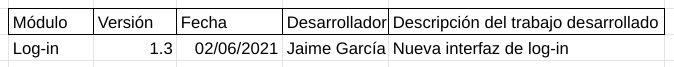
\includegraphics[height=1.3cm]{../images/tabla_versionado_code.png}
    \caption{Tabla de versionado del código.}
    \label{tablaVersionado}
\end{figure}

\begin{figure}[H]
    \centering
        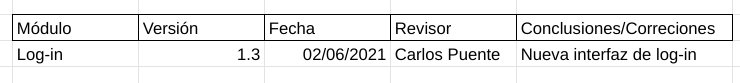
\includegraphics[height=1.5cm]{../images/tabla_conclusiones_revision_pares.png}
    \caption{Tabla de conclusiones de revisión por pares de código.}
    \label{tablaConclusionesPares}
\end{figure}

\underline{Revisión de los requisitos:}

Para comprobar el correcto cumplimiento de los requisitos del sistema se utilizará una tabla de cumplimiento de requisitos. 
En este tipo de revisión tanto el desarrollador como el revisor rellenarán dicha tabla y discutirán los resultados. 
Dichos resultados serán recogidos en una tabla de resumen que servirá como para futuras revisiones.
Los módulos de software a desarrollar anteriormente van asociados a ciertos requisitos del sistema. 
Antes de comenzar el desarrollo de un módulo se concretarán los requisitos finales a los que hace referencia 
y se generará la plantilla de la tabla de adecuación de requisitos.
Como en el modelo de revisión anterior, cuando el desarrollador del módulo termine una versión importante o 
realice un avance crítico solicitará una revisión al gestor del proyecto este le asignará un revisor adecuado para la tarea. 

\begin{figure}[H]
    \centering
        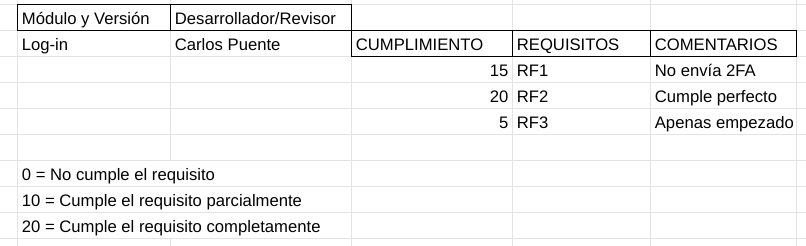
\includegraphics[height=4cm]{../images/tabla_cumplimiento_requisitos.png}
    \caption{Tabla de cumplimiento de requisitos.}
    \label{tablaRequisitos}
\end{figure}

\begin{figure}[H]
    \centering
        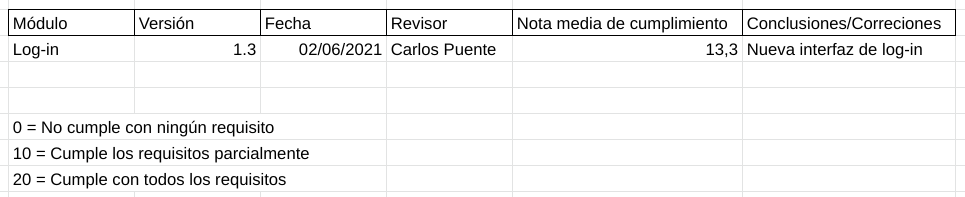
\includegraphics[height=3cm]{../images/tabla_conclusiones_revision_requisitos.png}
    \caption{Tabla de conclusiones de revisión de cumplimiento de requisitos.}
    \label{tablaConclusionesRequisitos}
\end{figure}

Todas estas tablas generadas por el proceso de aseguramiento de la calidad quedarán almacenadas en un directorio 
remoto accesible por todos los miembros del equipo de desarrollo agrupadas por el módulo al que hacen referencia 
de manera que sirvan como histórico de las revisiones realizadas y como mecanismo de monitorización del progreso
de las tareas.

\underline{Test sobre el producto: }

Para asegurar el funcionamiento correcto del código desarrollado se realizarán pruebas de desarrollo sobre los módulos, 
las cuales consistirán en pruebas unitarias y pruebas de integración con el resto de componentes del sistema. 
Además, una vez el sistema sea funcional, se realizarán pruebas globales sobre el sistema, las cuales consistirán en 
pruebas funcionales, de comunicación, de rendimiento, de sobrecarga… etc. 
Por último, utilizando las herramientas de despliegue continuo mencionadas anteriormente, se implementarán tests básicos 
sobre el sistema previos al despliegue.

\subsubsection{Calendario del proyecto y división del trabajo}

La división del trabajo se consiste en la partición del trabajo en los siguientes módulos:

Módulo de gestión de sign-ups de usuarios, módulo de gestión de log-ins de usuarios, 
módulo de gestión del Two-Factor-Authentication, módulo de generación de contraseñas, módulo de ranking de 
robustez de contraseñas, módulo de almacenamiento de contraseñas e información por usuario, módulo de búsqueda 
y ordenación de contraseñas y módulo de gestión y actualización de contraseñas e información. La documentación 
será del proyecto será actualizada por cada grupo de trabajo usando las \textit{Wikis} de \textit{GitHub} después de 
cada sesión de trabajo, del tal manera que los avances realizados en el desarrollo queden registrados haciendo 
posible el seguimiento del desarrollo al resto del equipo.
El diseño gráfico será realizado por todos los miembros del equipo mediante la creación de un \textit{mockup} 
de la misma en una reunión conjunta. 
Las instalaciones y los despliegues serán automáticos y continuos mediante \textit{scripts} de \textit{GitHub actions}. 
Las pruebas (Pruebas de desarrollo sobre los módulos y pruebas globales sobre el sistema) se realizarán conforme 
los desarrolladores vayan terminando sus designaciones y serán los mismos desarrolladores los cuales pasarán las 
pruebas, en el punto 3.2.3 se explica en detalle este aspecto. 

\pagebreak

\section{Análisis y diseño del sistema}

\subsection{Análisis de requisitos}

\begin{table}[H]
    \centering
    \begin{tabular}{| c | p{30em} |}
    \hline
        Código &  Descripción  \\ \hline
        RF-1 & El sistema permite almacenar contraseñas. \\ \hline
        RF-1.1 & El sistema permite almacenar pares que constan de nombre de usuario y contraseña.  \\ \hline
        RF-1.2 & Las entradas de contraseñas tienen un nombre asociado. \\ \hline
        RF-1.3 & El sistema permite asociar a las contraseñas una URL del sitio web al que corresponden. \\ \hline
        RF-1.4 & El sistema registra la fecha de creación y actualización de la contraseña. \\ \hline
        RF-1.5 & El sistema permite almacenar una descripción de texto asociada a la contraseña. \\ \hline
        RF-1.6 & El sistema permite almacenar ficheros de imagen (jpeg, png, ...) y ficheros PDF, asociados a la contraseña. \\ \hline
        RF - & El sistema asocia cada contraseña a una categoría del usuario\\ \hline
        RF - & El usuario puede crear, renombrar y eliminar categorías \\ \hline
        RF-2 & El sistema permite ordenar las contraseñas por categorías, fecha de creación y actualización. \\ \hline
        RF- & El sistema permite la visualización de las entradas de contraseña y todos sus datos y ficheros asociados.\\ \hline
        RF-3 & El sistema permite realizar una búsqueda entre las contraseñas por categoría, nombre de usuario.  \\ \hline
        RF-4 & El sistema permite generación de contraseñas pseudoaleatorias. \\ \hline
        RF-4.1 & El sistema permite seleccionar la longitud de la contraseña a generar.\\ \hline
        RF-4.2 & El sistema permite seleccionar el conjunto de caracteres que compone la contraseña a generar.\\ \hline
        RF-4.3 & El sistema mostrará el grado de robustez de la contraseña al ser generada. \\ \hline
        RF- & El usuario inicia sesión al sistema mediante su correo electrónico y la contraseña maestra. Únicamente podrá acceder con esta contraseña, que no se puede recuperar.\\ \hline
        RF-6 & El sistema requiere 2FA para iniciar sesión desde un dispositivo nuevo, distinto a los utilizados con anterioridad. \\ \hline
        RF- & El sistema permite el registro de un usuario con: correo electrónico, contraseña maestra, nombre, apellidos,... \textbf{MAS??}\\ \hline %% // TODO más??
        RF-7.1 & El registro de sesión se deberá confirmar, para verificar la identidad, mediante un correo al usuario registrado. \\ \hline
        RF- & La interfaz web permite copiar al cortapapeles del dispositivo la contraseña de una entrada. \textbf{sólo Web??}\\ \hline %% // TODO solo al web??
        RF-8 & El sistema permite la modificación de todos los campos de las contraseñas. \\ \hline
        RF-9 & Se accede al sistema mediante una aplicación móvil. \\ \hline
        RF-10 & Se accede al sistema mediante una interfaz web. \\ \hline
        RF-10 & El sistema ofrece un \textit{plug-in} para navegador web. \\ \hline
    \end{tabular}
\end{table}

\subsection{Diseño del sistema}


\section{Memoria del proyecto}

\subsection{Inicio del proyecto}

\subsection{Ejecución y control del proyecto}

\subsection{Cierre del proyecto}

\section{Conclusiones}

\section*{Glosario}
\addcontentsline{toc}{section}{Glosario}

\section*{Anexo I. Actas de todas las reuniones realizadas}
\addcontentsline{toc}{section}{Anexo I. Actas de todas las reuniones realizadas}

\section{Conclusiones}

\section{Bibliografía}

\end{document}
